% ==========================================================================
\chapter{耦合刚性稳定性分析}
% ==========================================================================

本章是全文的理论核心。第 \ref{sec:linearization} 节对半离散格式作线性化，得到显式与隐式算子的 Fourier 符号；第 \ref{sec:two-var-R} 节定义双变量稳定性函数并给出其几何解释；第 \ref{sec:admissible} 节给出容许分裂的严格定义；第 \ref{sec:main-theorem} 节证明纯耗散情形的精确条件 $\theta\le1/2$；第 \ref{sec:coupled-ratio} 节引入耦合刚性比，给出对流—扩散联合稳定域；第 \ref{sec:L-stability} 节讨论 L-稳定与刚性衰减；第 \ref{sec:discrete-symbol} 节把分析推广到全离散符号；第 \ref{sec:discussion} 节讨论结果的含义与局限。

\section{线性化与 Fourier 符号}
\label{sec:linearization}

考虑周期区间上的光滑解，将其在常数状态 $\bar u$ 附近展开：
\begin{equation}
  u_j(t)=\bar u+\delta u_j(t),\qquad |\delta u_j|\ll1.
\end{equation}
对一阶 Rusanov 格式，对流项 $f(u)=u^2/2$ 的导数为 $f'(\bar u)=\bar u\equiv a$，局部波速 $\alpha=|\bar u|=|a|$。线性化后的半离散系统为
\begin{equation}
\begin{split}
  \frac{\dd\,\delta u_j}{\dd t}
  &=-a\frac{\delta u_{j+1}-\delta u_{j-1}}{2\Delta x}
  +\frac{|a|}{2\Delta x}\left(\delta u_{j+1}-2\delta u_j+\delta u_{j-1}\right)\\
  &\quad+\frac{\nu}{\Delta x^2}\left(\delta u_{j+1}-2\delta u_j+\delta u_{j-1}\right).
\end{split}
  \label{eq:linearized-scheme}
\end{equation}
代入 Fourier 模态 $\delta u_j^n=\hat u^n\ee^{\ii kx_j}$，并记 $\xi=k\Delta x\in[0,\pi]$，得到
\begin{equation}
  \hat u^{n+1}=\left[1+\Delta t\left(\lambda_C(\xi)+\theta\nu\lambda_D(\xi)\right)\right]\hat u^n
  +\Delta t(1-\theta)\nu\lambda_D(\xi)\hat u^{n+1},
  \label{eq:fourier-imex}
\end{equation}
其中
\begin{equation}
  \lambda_C(\xi)=-\frac{\ii a\sin\xi}{\Delta x}
  -\frac{|a|(1-\cos\xi)}{\Delta x},
  \qquad
  \lambda_D(\xi)=-\frac{2(1-\cos\xi)}{\Delta x^2}.
  \label{eq:symbols}
\end{equation}
在长波极限 $\xi\to0$ 下，
\begin{equation}
  \lambda_C(\xi)=-\ii ak-\frac{|a|}{2}k^2\Delta x+O(\Delta x^2k^3),
  \qquad
  \lambda_D(\xi)=-k^2+O(\Delta x^2k^4).
  \label{eq:symbols-long-wave}
\end{equation}
与连续符号 $\lambda_C=-\ii ak$、$\lambda_D=-k^2$ 相比，离散对流符号多出一项 $-\frac{|a|}{2}k^2\Delta x$。这是 Rusanov 通量的数值耗散，其系数为 $|a|\Delta x/2$。它在下文中会略微放宽稳定域，但在 $\Delta x\to0$ 时消失。

定义
\begin{equation}
  z_E=\Delta t\left(\lambda_C+\theta\nu\lambda_D\right),
  \qquad
  z_I=\Delta t(1-\theta)\nu\lambda_D.
  \label{eq:zE-zI}
\end{equation}
由 \eqref{eq:fourier-imex} 得
\begin{equation}
  \hat u^{n+1}=R(z_E,z_I)\,\hat u^n,
  \qquad
  R(z_E,z_I)=\frac{1+z_E}{1-z_I}.
  \label{eq:R-def}
\end{equation}
稳定性要求对所有 $\xi\in[0,\pi]$ 都有 $|R(z_E(\xi),z_I(\xi))|\le1$。由于 $z_E$ 是复数而 $z_I$ 是实数（且非正），这是一个“复变量 $+$ 实参数”的稳定性问题。

为了把连续极限与离散计算区分开，本章同时使用两套符号。连续符号取 $\lambda_C=-\ii ak$、$\lambda_D=-k^2$，它给出干净的 $(\theta,d,\mu)$ 联合稳定域；离散符号 \eqref{eq:symbols} 多出 Rusanov 数值耗散，用于给出实际计算中的 CFL 型条件。两者的关系将在第 \ref{sec:discrete-symbol} 节说明。

\section{双变量稳定性函数}
\label{sec:two-var-R}

\begin{definition}[双变量稳定性函数]
  设 $z_E\in\mathbb{C}$，$z_I\in\mathbb{C}$，$z_I\ne1$。称
  \begin{equation}
    R(z_E,z_I)=\frac{1+z_E}{1-z_I}
    \label{eq:R-general}
  \end{equation}
  为 IMEX-Euler 的双变量稳定性函数。
\end{definition}

当 $z_I=0$ 时，$R=1+z_E$，退化为显式 Euler 的放大因子；当 $z_E=0$ 时，$R=1/(1-z_I)$，退化为隐式 Euler 的放大因子。因此，$R$ 是显式与隐式两种极限的统一推广。

\begin{lemma}[稳定域的圆盘表示]
  \label{lem:disk}
  设 $z_I\in\R$ 且 $z_I\le0$。则
  \begin{equation}
    |R(z_E,z_I)|\le1
    \iff
    |1+z_E|\le1-z_I.
    \label{eq:disk-condition}
  \end{equation}
  换言之，在复 $z_E$ 平面上，稳定域是以 $-1$ 为圆心、以 $1-z_I$ 为半径的闭圆盘。
\end{lemma}

\begin{proof}
  由 $z_I\le0$ 知 $1-z_I\ge1>0$，故
  \[
    |R|\le1
    \iff
    \frac{|1+z_E|}{|1-z_I|}\le1
    \iff
    |1+z_E|\le1-z_I.
  \]
  证毕。
\end{proof}

引理 \ref{lem:disk} 给出了一个非常直观的图像：随着 $|z_I|$ 增大，圆盘的半径 $1-z_I$ 线性增大，圆心固定在 $-1$。显式部分的贡献 $z_E$ 必须落在这个圆盘内，格式才稳定。对本文的分裂族，$z_E$ 与 $z_I$ 不是独立变化的，而是由同一个耗散算子按比例分配，因而在刚性极限下，$z_E$ 的模与圆盘半径以不同的速率增长。这正是耦合刚性问题的本质。

\section{容许分裂}
\label{sec:admissible}

在讨论具体条件之前，需要明确“容许分裂”的含义。直观上，一个分裂是容许的，如果隐式部分承载了足够的刚性，使得格式在刚性参数趋于无穷时仍然稳定。为了把它写成可检验的数学条件，引入如下定义。这里允许 $\theta=1$；此时隐式算子取为恒等算子，对应“没有隐式部分”的退化情形。

\begin{definition}[刚性射线]
  对纯耗散情形 $\lambda_C=0$，$\lambda_D=-k^2$，令
  \begin{equation}
    z_D=\Delta t\nu\lambda_D=-x,\qquad x\ge0.
    \label{eq:zD}
  \end{equation}
  则
  \begin{equation}
    z_E=-\theta x,\qquad z_I=-(1-\theta)x.
    \label{eq:stiff-ray}
  \end{equation}
  称集合
  \begin{equation}
    \mathcal{R}_\theta=\left\{\left(-\theta x,-(1-\theta)x\right):x\ge0\right\}
    \label{eq:ray-set}
  \end{equation}
  为分裂参数 $\theta$ 对应的刚性射线。
\end{definition}

\begin{definition}[容许分裂]
  \label{def:admissible}
  称分裂参数 $\theta\in[0,1]$ 是容许的，如果
  \begin{enumerate}[label=(\roman*),leftmargin=2.4em]
    \item 隐式算子 $\bI-(1-\theta)\nu\Delta t\bD$ 对任意 $\Delta t>0$ 可逆（当 $\theta=1$ 时约定为恒等算子）；
    \item 沿刚性射线一致稳定，即
    \begin{equation}
      \sup_{x\ge0}\left|R\left(-\theta x,-(1-\theta)x\right)\right|\le1.
      \label{eq:admissible-condition}
    \end{equation}
  \end{enumerate}
\end{definition}

条件 (i) 在 $\theta<1$ 时自动满足：$\bD$ 的特征值非正，故 $\bI-(1-\theta)\nu\Delta t\bD$ 正定；$\theta=1$ 时约定为恒等算子。真正排除 $\theta=1$ 的是条件 (ii)：此时没有隐式部分，格式退化为显式 Euler，对刚性扩散不可能稳定。

\begin{definition}[沿刚性射线的 L-稳定]
  若 $\theta$ 是容许的，且
  \begin{equation}
    \lim_{x\to\infty}R\left(-\theta x,-(1-\theta)x\right)=0,
    \label{eq:coupled-L}
  \end{equation}
  则称该分裂沿刚性射线是 L-稳定的。
\end{definition}

这里需要强调与经典 L-稳定的区别。经典定义固定 $z_E$、令 $z_I\to-\infty$，此时对任意 $\theta<1$ 都有 $R\to0$。但在耦合分裂中，$z_E$ 与 $z_I$ 同时趋于无穷，$z_E$ 的贡献不会被分母完全压制。因此，经典意义下的 L-稳定不足以刻画本文的问题；必须使用沿射线的极限 \eqref{eq:coupled-L}。这一细微差别是理解 $\theta=1/2$ 边界的关键。

\section{主要定理}
\label{sec:main-theorem}

\begin{theorem}[纯耗散情形的精确稳定性条件]
  \label{thm:main}
  设 $\theta\in[0,1]$，$x\ge0$，$R$ 由 \eqref{eq:R-general} 定义。则
  \begin{equation}
    \left|R\left(-\theta x,-(1-\theta)x\right)\right|\le1
    \iff
    (1-2\theta)x+2\ge0.
    \label{eq:main-ineq}
  \end{equation}
\end{theorem}

\begin{proof}
  沿刚性射线，
  \begin{equation}
    R\left(-\theta x,-(1-\theta)x\right)
    =\frac{1-\theta x}{1+(1-\theta)x}.
    \label{eq:R-ray}
  \end{equation}
  由于 $x\ge0$、$0\le\theta\le1$，分母 $1+(1-\theta)x>0$。于是
  \begin{align}
    |R|\le1
    &\iff (1-\theta x)^2\le\left(1+(1-\theta)x\right)^2 \notag\\
    &\iff 1-2\theta x+\theta^2x^2
    \le1+2(1-\theta)x+(1-\theta)^2x^2 \notag\\
    &\iff -2x\le\left[(1-\theta)^2-\theta^2\right]x^2 \notag\\
    &\iff -2x\le(1-2\theta)x^2 \notag\\
    &\iff x\left[(1-2\theta)x+2\right]\ge0. \label{eq:proof-last}
  \end{align}
  因 $x\ge0$，上式等价于 $(1-2\theta)x+2\ge0$。证毕。
\end{proof}

定理 \ref{thm:main} 的结论可以分两种情形表述。

\begin{corollary}
  \label{cor:cases}
  \begin{enumerate}[label=(\arabic*),leftmargin=2.4em]
    \item 若 $0\le\theta\le1/2$，则对任意 $x\ge0$ 都有 $|R|\le1$；
    \item 若 $1/2<\theta\le1$，则 $|R|\le1$ 当且仅当
    \begin{equation}
      x\le\frac{2}{2\theta-1}.
      \label{eq:finite-threshold}
    \end{equation}
  \end{enumerate}
\end{corollary}

\begin{proof}
  由定理 \ref{thm:main} 直接得到。当 $\theta\le1/2$ 时 $1-2\theta\ge0$，故 $(1-2\theta)x+2\ge2>0$；当 $\theta>1/2$ 时 $1-2\theta<0$，不等式化为 $x\le2/(2\theta-1)$。$\theta=1$ 时右端为 $2$，与 $|R|=|1-x|\le1$ 一致。
\end{proof}

推论 \ref{cor:cases} 给出了本文的第一个核心结论：
\begin{equation}
  \boxed{\ \theta\le\frac12\ }
  \label{eq:theta-half}
\end{equation}
是分裂族在耗散主导的耦合刚性极限下保持稳定的充要条件。当 $\theta>1/2$ 时，稳定性只能在一个有限的刚性范围内维持；一旦 $|z_D|$ 超过阈值 $2/(2\theta-1)$，格式必然失稳。阈值随 $\theta\to1/2^+$ 发散，随 $\theta\to1$ 减小到 $2$，与直觉一致。

\subsection{几何解释}

定理 \ref{thm:main} 有一个漂亮的几何证明。由引理 \ref{lem:disk}，对固定的 $x$，稳定域是圆盘
\begin{equation}
  D(x)=\left\{z_E:|z_E+1|\le1+(1-\theta)x\right\}.
\end{equation}
刚性射线上的点是 $z_E=-\theta x$，它到圆心的距离为
\begin{equation}
  |1-\theta x|,
\end{equation}
而圆盘半径为 $1+(1-\theta)x$。当 $x$ 很大时，距离的增长速率为 $\theta$，半径的增长速率为 $1-\theta$。因此，点能否留在圆盘内，取决于 $\theta$ 与 $1-\theta$ 的大小：
\begin{itemize}[leftmargin=2.2em]
  \item 若 $\theta<1/2$，距离增长得慢，点始终在圆盘内；
  \item 若 $\theta=1/2$，两者同速，点渐近地贴着圆盘边界；
  \item 若 $\theta>1/2$，距离增长得快，点终将穿出圆盘。
\end{itemize}
图 \ref{fig:stability-geometry}(a) 画出了 $x=10$ 时 $\theta=0.25$ 与 $\theta=0.75$ 对应的两个圆盘及射线上的点：前者在圆内，后者在圆外。图 \ref{fig:stability-geometry}(b) 则给出 $|R|$ 随 $x$ 的变化，虚线为各 $\theta$ 对应的极限值 $\theta/(1-\theta)$。可以看到，$\theta=0.5$ 的曲线恰好以 $1$ 为极限，$\theta>0.5$ 的曲线穿过 $1$ 并继续上升。

\begin{figure}[htbp]
  \centering
  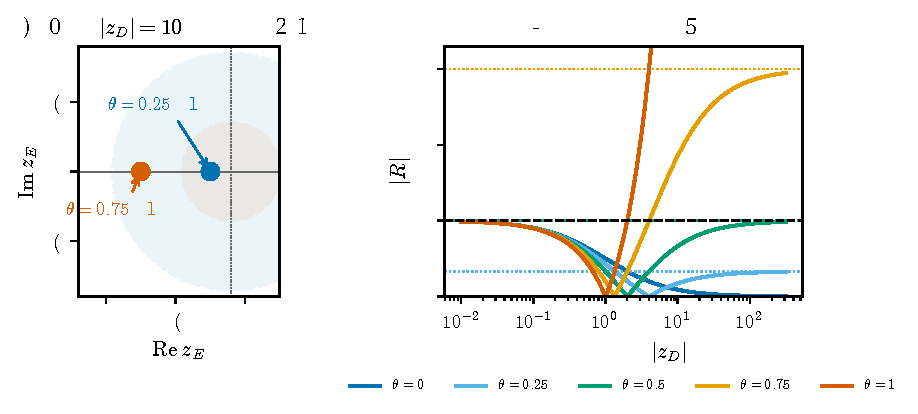
\includegraphics[width=0.96\textwidth]{stability_geometry.pdf}
  \caption{双变量稳定性函数的几何图像。(a) 固定 $|z_D|=10$ 时的稳定域圆盘与刚性射线上的点；(b) 沿刚性射线的放大因子，虚线为极限 $\theta/(1-\theta)$。}
  \label{fig:stability-geometry}
\end{figure}

图 \ref{fig:stability-region} 进一步给出了 $(\theta,\log_{10}|z_D|)$ 平面上的精确稳定域。黑色实线为 $|R|=1$ 的边界，其方程由 \eqref{eq:finite-threshold} 给出：
\begin{equation}
  \log_{10}|z_D|=\log_{10}\frac{2}{2\theta-1},\qquad \theta>\frac12.
  \label{eq:boundary-curve}
\end{equation}
$\theta\le1/2$ 的整个左半区域都是稳定的；$\theta>1/2$ 时，稳定域位于边界曲线下方。随着 $|z_D|$ 增大，允许的 $\theta$ 越来越接近 $1/2$。这张图可以看作分裂族的“相图”：它把稳定性问题转化为一个二维区域问题，便于设计参数。

\begin{figure}[htbp]
  \centering
  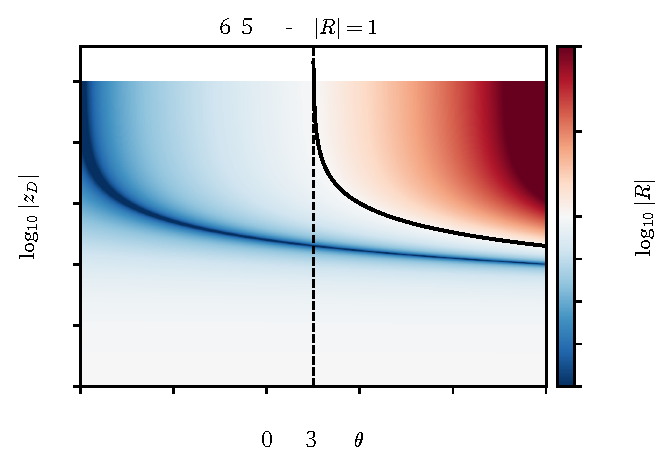
\includegraphics[width=0.72\textwidth]{stability_region.pdf}
  \caption{精确稳定域 $|R(z_E,z_I)|\le1$ 在 $(\theta,\log_{10}|z_D|)$ 平面上的相图。黑色实线为边界 \eqref{eq:boundary-curve}。}
  \label{fig:stability-region}
\end{figure}

\subsection{刚性极限}

由 \eqref{eq:R-ray}，当 $\theta<1$ 且 $x\to\infty$ 时
\begin{equation}
  \lim_{x\to\infty}R\left(-\theta x,-(1-\theta)x\right)
  =-\frac{\theta}{1-\theta}.
  \label{eq:R-infinity}
\end{equation}
其模为 $\theta/(1-\theta)$。条件 $|R_\infty|\le1$ 等价于 $\theta\le1/2$，与定理 \ref{thm:main} 一致。这个极限值有清晰的物理意义：在扩散主导的刚性极限下，显式部分把比例为 $\theta$ 的耗散“漏”了出去，隐式部分只能压住剩下的 $1-\theta$；两者之比决定了残余放大因子的幅度。

对 $\theta=1/2$，$R_\infty=-1$。这不是真正的衰减，而是每个时间步改变符号、幅度不变的寄生振荡。它在数值解中表现为网格尺度的锯齿波，虽然不发散，但会污染解的精度。这一点将在第五章的数值实验中得到验证。

\section{耦合刚性比与联合稳定域}
\label{sec:coupled-ratio}

\subsection{连续符号的联合稳定条件}

前面的定理只考虑了纯耗散情形 $\lambda_C=0$。实际计算中对流与扩散同时存在，因此需要把 $z_E$ 的实部（耗散）与虚部（对流）一起保留。对连续符号
\begin{equation}
  \lambda_C=-\ii ak,\qquad \lambda_D=-k^2,
\end{equation}
令
\begin{equation}
  \mu=ak\Delta t,\qquad d=\nu k^2\Delta t\ge0.
  \label{eq:mu-d}
\end{equation}
则
\begin{equation}
  z_E=-\ii\mu-\theta d,\qquad z_I=-(1-\theta)d.
  \label{eq:zE-continuous}
\end{equation}
代入 \eqref{eq:R-general} 得
\begin{equation}
  R=\frac{1-\theta d-\ii\mu}{1+(1-\theta)d}.
  \label{eq:R-continuous}
\end{equation}
稳定性条件 $|R|\le1$ 等价于
\begin{equation}
  (1-\theta d)^2+\mu^2\le\left(1+(1-\theta)d\right)^2.
  \label{eq:continuous-ineq}
\end{equation}
展开并整理，得到本文的第二个核心结论：
\begin{equation}
  \boxed{\ \mu^2\le 2d+(1-2\theta)d^2\ }.
  \label{eq:coupled-condition}
\end{equation}
当 $\mu=0$ 时，\eqref{eq:coupled-condition} 化为 $d[(1-2\theta)d+2]\ge0$，即定理 \ref{thm:main} 中的 $(1-2\theta)d+2\ge0$。因此，纯耗散定理是联合稳定条件在 $\mu=0$ 处的切片。

对固定的 $\theta$ 与 $d$，允许的对流强度为
\begin{equation}
  |\mu|\le\mu_{\max}(d)
  =\sqrt{\max\left\{0,\ 2d+(1-2\theta)d^2\right\}}.
  \label{eq:mu-max}
\end{equation}
当 $\theta\le1/2$ 时，根号内的二次式对一切 $d\ge0$ 非负，稳定域向 $d$ 方向无限延伸；当 $\theta>1/2$ 时，二次式在
\begin{equation}
  d>d_c=\frac{2}{2\theta-1}
  \label{eq:dc}
\end{equation}
时变负，此时即使 $\mu=0$ 也不稳定，这与定理 \ref{thm:main} 的有限阈值完全一致。

在长波极限 $d\to0$ 下，$\mu_{\max}\approx\sqrt{2d}$，与 $\theta$ 无关；在 $d\to\infty$ 时，
\begin{equation}
  \mu_{\max}\sim
  \begin{cases}
    \sqrt{1-2\theta}\,d, & \theta<1/2,\\[4pt]
    \sqrt{2d}, & \theta=1/2.
  \end{cases}
  \label{eq:mu-asymptotic}
\end{equation}
这说明：当隐式部分至少承担一半耗散时，对流可以按 $O(d)$ 的速度增长而不破坏稳定性；当 $\theta=1/2$ 时，对流的容许量只按 $\sqrt d$ 增长；当 $\theta>1/2$ 时，稳定域在 $d_c$ 处终止。

\subsection{耦合刚性比与 \texorpdfstring{$\beta_\infty(\varepsilon)$}{beta-inf}}

联合稳定条件还可以用“刚性比”的语言表述。设 $z_E$ 与 $z_I$ 按固定比例同时趋于无穷：
\begin{equation}
  z_I=\varepsilon z_E,\qquad |z_E|\to\infty,\qquad \varepsilon\ne0.
  \label{eq:epsilon-def}
\end{equation}
则
\begin{equation}
  R=\frac{1+z_E}{1-\varepsilon z_E}
  \longrightarrow
  \beta_\infty(\varepsilon)=-\frac{1}{\varepsilon}.
  \label{eq:beta-infinity}
\end{equation}
称 $\beta_\infty(\varepsilon)$ 为耦合刚性极限的放大因子。格式在该极限下稳定，当且仅当
\begin{equation}
  |\beta_\infty(\varepsilon)|\le1
  \iff
  |\varepsilon|\ge1.
  \label{eq:epsilon-stable}
\end{equation}
对本文的 $\theta$ 族，沿纯耗散射线有
\begin{equation}
  \varepsilon=\frac{z_I}{z_E}=\frac{1-\theta}{\theta},
  \qquad \theta\in(0,1].
  \label{eq:epsilon-theta}
\end{equation}
于是
\begin{equation}
  |\varepsilon|\ge1
  \iff
  \frac{1-\theta}{\theta}\ge1
  \iff
  \theta\le\frac12,
  \label{eq:epsilon-half}
\end{equation}
与 \eqref{eq:theta-half} 完全一致。这个推导把“显式与隐式各承担多少”翻译成一个无量纲比值：$\varepsilon$ 越大，隐式部分相对越强；$\varepsilon=1$ 是临界点，$\varepsilon<1$ 时显式部分过强，刚性极限下的残余放大因子的模超过 $1$。当 $\theta=1$ 时 $\varepsilon=0$，没有隐式部分，$R=1+z_E$ 无界，不属于上述极限。

需要强调，$\beta_\infty(\varepsilon)$ 是 IMEX-Euler 的普适函数，与具体的空间算子无关；分裂族只负责在曲线 $\varepsilon=(1-\theta)/\theta$ 上选点。这一观点把“设计分裂”转化为“在 $|\beta_\infty(\varepsilon)|\le1$ 的区域内选 $\varepsilon$”，比逐点检查 $|R|$ 更便于推广到其他格式。

\subsection{几何图像}

图 \ref{fig:stability-coupled}(a) 画出了 $\mu_{\max}(d)$ 随 $d$ 的变化。曲线下方为稳定区，上方为不稳定区；$\theta>1/2$ 的曲线在 $d_c$ 处终止。图 \ref{fig:stability-coupled}(b) 画出了 $|\beta_\infty(\varepsilon)|=1/|\varepsilon|$，并标出了 $|\varepsilon|\ge1$ 的稳定侧。两张图从不同角度描述同一件事：稳定性由“显式部分与隐式部分的相对强度”决定，而不是由某一个单独的稳定性参数决定。

\begin{figure}[htbp]
  \centering
  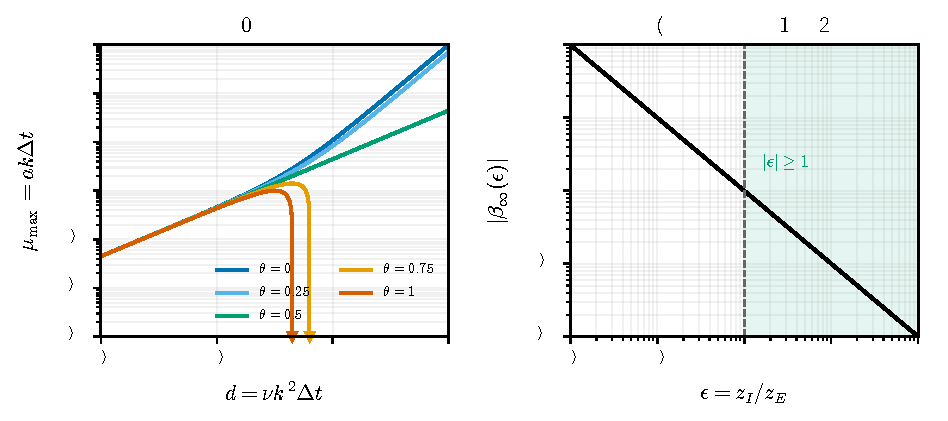
\includegraphics[width=0.96\textwidth]{stability_coupled.pdf}
  \caption{连续符号下的联合稳定域。(a) 曲线 $\mu_{\max}(d)$ 下方为稳定区；$\theta>1/2$ 时曲线在 $d=2/(2\theta-1)$ 处终止。(b) 刚性极限放大因子 $|\beta_\infty(\varepsilon)|=1/|\varepsilon|$；$|\varepsilon|\ge1$ 时不超过 $1$。}
  \label{fig:stability-coupled}
\end{figure}

图 \ref{fig:stability-coupled}(a) 还揭示了两种不同的失稳机制。第一种是“耗散不足”：当 $\theta>1/2$ 且 $d>d_c$ 时，隐式部分压不住显式耗散，纯耗散模态本身就不稳定；第二种是“对流—扩散失衡”：当 $d$ 较小而 $\mu$ 较大时，显式对流项超出圆盘所能容纳的范围。前者由 $\theta$ 控制，后者由 $\mu/d$ 控制。第 \ref{sec:discrete-symbol} 节将说明，离散格式的网格尺度失稳属于第一种机制，而长波失稳属于第二种机制。

\section{L-稳定与刚性衰减}
\label{sec:L-stability}

\begin{table}[htbp]
  \centering
  \small
  \setlength{\tabcolsep}{5pt}
  \caption{不同 $\theta$ 的稳定性性质}
  \label{tab:theta-stability}
  \begin{tabular}{lcccc}
    \toprule
    $\theta$ & $R_\infty$ & 刚性稳定 & L-稳定 & 表现 \\
    \midrule
    $0$ & $0$ & 所有 $x$ & 是 & 强阻尼 \\
    $(0,\frac12)$ & $-\frac{\theta}{1-\theta}$ & 所有 $x$ & 否 & 有界振荡 \\
    $\frac12$ & $-1$ & 所有 $x$ & 否 & 临界振荡 \\
    $(\frac12,1)$ & $|R_\infty|>1$ & $x\le\frac{2}{2\theta-1}$ & 否 & 大 $x$ 失稳 \\
    $1$ & $-\infty$ & $x\le2$ & 否 & 条件稳定 \\
    \bottomrule
  \end{tabular}
\end{table}

表 \ref{tab:theta-stability} 汇总了各种情形的稳定性。可以得到如下结论。

第一，只有 $\theta=0$ 是沿刚性射线 L-稳定的。此时 $R=1/(1+x)\to0$，最快的耗散模态被完全压掉。这与经典理论中“全隐式 Euler 是 L-稳定的”一致。

第二，$0<\theta\le1/2$ 沿刚性射线稳定，但不是 L-稳定的。其极限放大因子为 $-\theta/(1-\theta)$，绝对值小于 $1$（$\theta=1/2$ 时等于 $1$）。这意味着格式不会发散，但也不会把刚性模态完全衰减；在长时间计算中，这些模态可能以低频振荡的形式残留。

第三，$\theta=1/2$ 是临界情形。它恰好满足 $|R_\infty|=1$，属于“中性稳定”。它没有稳定裕度；在非线性计算中，若同时存在其他失稳机制（例如边界反射、限制器开关），可能表现为网格尺度的弱振荡。因此，在实际计算中不宜把 $\theta=1/2$ 当作安全边界：它是理论上的分界点，而不是工程上的推荐值。

第四，$\theta>1/2$ 只在一个有限的刚性范围内稳定。随着网格加密或 $\nu$ 增大，$|z_D|$ 增大，格式终将失稳。这一结论对时间步长控制有直接影响：不能简单地用 CFL 条件来选取 $\Delta t$，还必须考虑扩散刚性。

\section{离散符号与 CFL 条件}
\label{sec:discrete-symbol}

定理 \ref{thm:main} 与联合条件 \eqref{eq:coupled-condition} 是对连续符号的结论。实际计算使用的是全离散格式，其稳定性由 \eqref{eq:symbols} 的离散符号决定。本节给出离散情形的分析，并说明它与连续结论的关系。

\subsection{全离散放大因子}

将 \eqref{eq:symbols} 代入 \eqref{eq:zE-zI}，记
\begin{equation}
  c=\frac{a\Delta t}{\Delta x},\qquad
  r=\frac{\nu\Delta t}{\Delta x^2},\qquad
  q=1-\cos\xi\in[0,2],
  \label{eq:c-r-q}
\end{equation}
并令
\begin{equation}
  \delta=cq,\qquad \mu=c\sin\xi,\qquad d=2rq.
  \label{eq:delta-mu-d}
\end{equation}
则
\begin{equation}
  z_E=-\delta-\theta d-\ii\mu,
  \qquad
  z_I=-(1-\theta)d,
  \label{eq:zE-discrete}
\end{equation}
放大因子为
\begin{equation}
  R(\xi)=\frac{1-\delta-\theta d-\ii\mu}{1+(1-\theta)d}.
  \label{eq:R-discrete}
\end{equation}
稳定性条件 $|R(\xi)|\le1$ 对任意 $\xi\in[0,\pi]$ 成立。直接对 $\xi$ 扫描即可得到数值稳定域；下面给出两个有解析表达的极端情形。

\subsection{网格尺度分析}

在网格尺度 $\xi=\pi$ 处，$q=2$，$\delta=2c$，$\mu=0$，$d=4r$。代入 \eqref{eq:R-discrete} 得
\begin{equation}
  z_E=-2c-4\theta r,\qquad z_I=-4(1-\theta)r,
  \label{eq:sawtooth}
\end{equation}
稳定性条件为
\begin{equation}
  \left|1-2c-4\theta r\right|\le1+4(1-\theta)r.
  \label{eq:sawtooth-ineq}
\end{equation}
对 $\theta>1/2$ 且 $r$ 较大，左端为 $2c+4\theta r-1$，右端为 $1+4(1-\theta)r$，于是
\begin{equation}
  2c+4(2\theta-1)r\le2
  \iff
  c+2(2\theta-1)r\le1.
  \label{eq:sawtooth-condition}
\end{equation}
这就是 $\theta>1/2$ 时的扩散限制。几个特例如下：
\begin{align}
  \theta=1:&\qquad c+2r\le1; \label{eq:theta1-cfl}\\
  \theta=3/4:&\qquad c+r\le1; \label{eq:theta34-cfl}\\
  \theta=1/2:&\qquad c\le1. \label{eq:theta12-cfl}
\end{align}
当 $c$ 很小时（扩散主导），\eqref{eq:theta1-cfl} 给出 $r\le1/2$，即 $\Delta t\le\Delta x^2/(2\nu)$，这正是显式扩散的标准稳定性条件。对 $\theta=3/4$，条件放宽为 $r\le1$；对 $\theta=1/2$，扩散限制消失，只剩下 CFL 条件 $c\le1$。

\subsection{长波分析与数值耗散}

对 $\theta\le1/2$，网格尺度是稳定的（$\theta<1/2$）或退化为 $c\le1$（$\theta=1/2$），此时限制可能来自长波。把 \eqref{eq:symbols-long-wave} 代入连续稳定性条件，等价地，在 \eqref{eq:R-discrete} 中令 $\xi\to0$。由
\begin{equation}
  \delta\approx\frac{c}{2}\xi^2,\qquad
  d\approx r\xi^2,\qquad
  \mu\approx c\xi,
\end{equation}
并只保留 $\xi^2$ 阶项，\eqref{eq:R-discrete} 的稳定性条件给出
\begin{equation}
  c^2\le c+2r.
  \label{eq:long-wave-c-r}
\end{equation}
把 $c=a\Delta t/\Delta x$、$r=\nu\Delta t/\Delta x^2$ 代入，整理得
\begin{equation}
  \Delta t\le\frac{2\nu+|a|\Delta x}{a^2}.
  \label{eq:low-k-numerical}
\end{equation}
若忽略 Rusanov 的数值耗散（即把 $|a|\Delta x$ 项去掉），则回到
\begin{equation}
  \Delta t\le\frac{2\nu}{a^2}.
  \label{eq:low-k-condition}
\end{equation}
注意这个条件与 $\Delta x$ 无关，它是一个“扩散时间尺度”条件，而不是 CFL 条件。当 $\nu$ 较大时，它允许较大的 $\Delta t$；当 $\nu$ 较小时，它变得严格。

条件 \eqref{eq:long-wave-c-r} 有一个重要的推论：当 $\theta<1/2$ 时，隐式扩散足够强，CFL 数可以远大于 $1$。例如取 $\nu=1$、$a=1$、$\Delta x=0.005$，\eqref{eq:low-k-numerical} 给出 $\Delta t\lesssim2.005$，对应的 $c\approx401$。这解释了第五章中 $\theta=0$ 与 $\theta=1/4$ 的最大步长约为 $2.05$ 的现象：限制来自扩散时间尺度，而不是对流 CFL 条件。对 $\theta=1/2$，网格尺度条件 \eqref{eq:theta12-cfl} 给出 $\Delta t\le\Delta x/a$，它比 \eqref{eq:low-k-numerical} 更严格，因此最大步长在 $\theta=1/2$ 处出现断崖式下降。

图 \ref{fig:stability-discrete} 给出了固定 $\CFL=0.4$、$\nu=1$、$N=200$ 时 $|R(\xi)|$ 随 $\xi$ 的变化。此时 $\nu\Delta t/\Delta x^2=80$，属于强扩散情形。$\theta=0$、$0.25$、$0.5$ 的曲线始终不超过 $1$；$\theta=0.6$、$0.75$、$1$ 的曲线在某个波数之后穿过 $1$，并迅速上升（$\theta=1$ 更早，因为全部耗散都在显式部分）。这正是 $\theta>1/2$ 时网格尺度失稳的直接证据，也是 \eqref{eq:sawtooth-condition} 中 $r$ 项占主导的体现。

\begin{figure}[htbp]
  \centering
  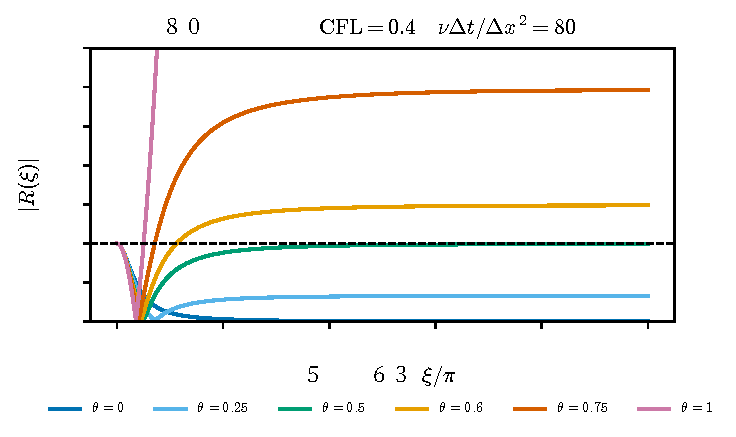
\includegraphics[width=0.78\textwidth]{stability_discrete.pdf}
  \caption{全离散放大因子 $|R(\xi)|$ 随无量纲波数的变化（$\CFL=0.4$，$\nu\Delta t/\Delta x^2=80$）。虚线为 $|R|=1$。}
  \label{fig:stability-discrete}
\end{figure}

\subsection{离散稳定性的完整图像}

综合以上分析，离散格式的稳定性可以概括为：

\begin{enumerate}[label=(\roman*),leftmargin=2.4em]
  \item 当 $\theta<1/2$ 时，网格尺度无条件稳定；时间步长由长波条件 \eqref{eq:low-k-numerical} 控制。此时 CFL 数可以大于 $1$，甚至远大于 $1$，但格式的精度会下降。
  \item 当 $\theta=1/2$ 时，网格尺度条件退化为 $c\le1$，长波条件仍为 \eqref{eq:low-k-numerical}；最大步长由两者中较小者决定。对本文的参数（$\nu=1$，$N=200$），$c\le1$ 是起决定作用的约束，因此 $\Delta t_{\max}=\Delta x$。
  \item 当 $\theta>1/2$ 时，除长波条件外，还必须满足网格尺度条件 \eqref{eq:sawtooth-condition}。随着 $\theta\to1$，该条件趋于 $c+2r\le1$，即显式扩散的经典限制。
  \item 无论 $\theta$ 取何值，$\Delta t$ 都不能由单一的 CFL 条件确定；必须同时检查 $c$、$r$ 与刚性参数 $z_D$。
\end{enumerate}

\section{讨论}
\label{sec:discussion}

\subsection{为什么边界是 \texorpdfstring{$1/2$}{1/2}}

定理 \ref{thm:main} 的证明只用了初等代数，但 $1/2$ 的出现并非偶然。在刚性射线上，显式部分承担的耗散比例为 $\theta$，隐式部分为 $1-\theta$。当 $x\to\infty$ 时，显式部分的放大因子为 $-\theta x$，隐式部分的分母为 $(1-\theta)x$。两者之比为 $-\theta/(1-\theta)$。要求其模不超过 $1$，自然得到 $\theta\le1/2$。从几何上看，这是射线斜率 $\theta$ 与圆盘半径斜率 $1-\theta$ 的竞争。因此，$1/2$ 是“显式与隐式各承担一半”的临界点，具有明确的物理意义。

\subsection{与 Zakerzadeh--Noelle 判据的关系}

Zakerzadeh 与 Noelle 在研究刚性双曲守恒律的 IMEX 通量分裂时，系统比较了对称分裂与非对称分裂：对称分裂可以做到对刚性参数一致稳定，而非对称分裂不一定；他们通过具体算例说明，某些看似自然的分裂会出现小范围的不稳定\cite{zakerzadeh2018}。用本文的语言，这说明“把刚性项放进隐式部分”只是容许性的必要条件，而不是充分条件；分裂的对称性与结构同样重要。本文的 $\theta$ 族是非对称分裂，因此需要逐点分析；定理 \ref{thm:main} 给出的 $\theta\le1/2$ 正是这种分析的结果。与他们的判据相比，本文的结论更细：$\theta\le1/2$ 虽然不是 L-稳定的，但沿刚性射线仍然是稳定的；它在有限刚性下可用，只是在极强的刚性下会留下不衰减的残余模态。

\subsection{线性分析的局限}

本章的分析基于线性化与冻结系数。对非线性 Burgers 方程，激波附近的系数变化、限制器的开关、边界条件等都可能影响稳定性。线性分析给出的是必要条件：如果线性化格式不稳定，非线性格式必然不稳定；反之，线性稳定并不保证非线性稳定。因此，第五章的数值实验不仅是对理论的验证，也是对非线性效应的补充。实验中采用的 MUSCL/minmod 重构具有 TVD 性质，可以在一定程度上抑制非线性振荡；但限制器在极值点附近退化为一阶，也会影响精度。这些因素在解读实验结果时都需要考虑。

\subsection{稳定性与精度的张力}

从表 \ref{tab:theta-stability} 可以看到，$\theta=0$ 具有最好的稳定性，但它的隐式部分最“重”；$\theta=1/2$ 的计算最便宜（隐式部分只有一半），但处于临界状态。稳定性与精度并不是同一个问题：一个格式可以稳定但过度耗散，也可以精确但脆弱。第五章将用激波算例说明，在稳定的前提下，$\theta$ 对精度的影响是温和的；真正决定精度的是空间格式的阶数与数值耗散，而不是 $\theta$ 本身。

\section{本章小结}

本章建立了参数化分裂族的稳定性理论。主要结果包括：
\begin{enumerate}[label=(\arabic*),leftmargin=2.4em]
  \item 双变量稳定性函数 $R(z_E,z_I)=(1+z_E)/(1-z_I)$ 及其圆盘表示；
  \item 纯耗散情形下的精确条件 $(1-2\theta)x+2\ge0$，即 $\theta\le1/2$ 时对所有刚性稳定，$\theta>1/2$ 时仅对 $x\le2/(2\theta-1)$ 稳定；
  \item 连续符号下的联合稳定条件 $\mu^2\le2d+(1-2\theta)d^2$，以及刚性比表述 $|\beta_\infty(\varepsilon)|=1/|\varepsilon|$，$|\varepsilon|\ge1$；
  \item 只有 $\theta=0$ 沿刚性射线 L-稳定，$\theta=1/2$ 是临界稳定；
  \item 全离散符号分析给出了 $\theta>1/2$ 时的网格尺度条件 $c+2(2\theta-1)r\le1$，以及长波条件 $\Delta t\le(2\nu+|a|\Delta x)/a^2$。
\end{enumerate}
这些结果为第五章的数值验证提供了明确的可检验预测。
